\section{exampels}

\paragraph{VC dimension}

To illustrate this concept intuitively, consider the simple function class of one-dimensional intervals on the real line. 
In this case, the VC dimension can be easily grasped. 
Let $\mathcal{H}$ be the set of all intervals of the form $[a, b]$, where $a$ and $b$ are real numbers. An interval classifier labels by $1$ any point which lays inside the interval and $0$ for any other point.
It is clear that if we take two distinct points $x_1$ and $x_2$ in the real line such that, w.l.o.g, $x_1 < x_2$, we can find intervals in $\mathcal{H}$ that can shatter them. spesifically: 
\begin{intemize}
  \item The interval $[x_1-2,x_1-1]$ labels the pair by $(0,0)$.
  \item The interval $[x_1-1,x_1]$ labels the pair by $(0,1)$.
  \item The interval $[x_2+1,x_2+2]$ labels the pair by $(1,1)$.
  \item The interval $[x_2,x_2+1]$ labels the pair by $(1,0)$.
\end{itemize}
In other words the pair $x_1$ and $x_2$ can be labeled by any possible sequence of binary sequence of the same length. 
But, given a triplet $x_1 < x_2 < x_3$ there is not interval in $\mathcal{H}$ that can label them $(1,0,1)$.
As the size of the smallest set that can be shattered by $\mathcal{H}$ is $2$, the VC dimension of $\mathcal{H}$ is $2$. 

\paragraph{Fat-shattering dimension}
To demonstrate this concept intuitively, consider the class of affine functions on the real line. Given a pair of points $x_1$ and $x_2$ the pair is $\gamma$-shattered by the class for any given $\gamma$. A visual illustration of this is given in Figure~\ref{fig:fat-shattering} on which two example points $x_1,x_2$ are given and the $4$ affine functions shatter the pair (each function labeled by the resulting pair's labeling) and the points $r_1,r_2$ witness the shattering as described in the above definition.  
% The name of the figure file is shattering.png
\begin{figure}[h]
  \centering
  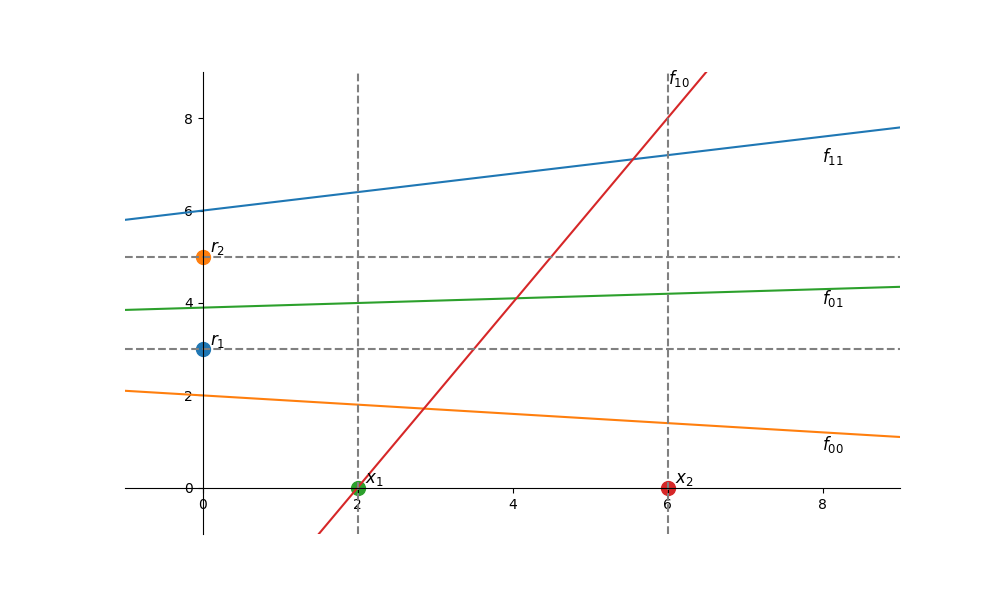
\includegraphics[width=0.5\textwidth]{shattering.png}
  \caption{Fat-shattering illustration}
  \label{fig:fat-shattering}
\end{figure}
